\section{Work To Date}

The application displays metabolic pathway graphs for all pathways for which PathCase provides a static layout. These graphs can be navigated by panning and zooming. A screenshot of the interface is shown in figure \ref{fig:screenshot}

\begin{figure}[htb]
    \center{
        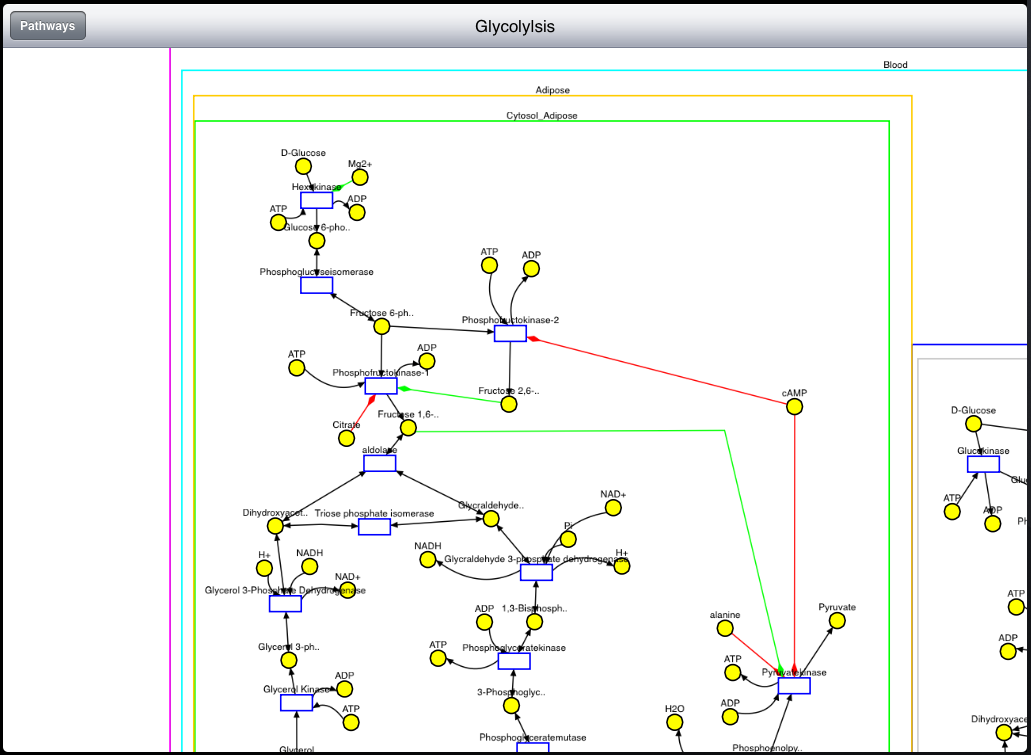
\includegraphics[width=4in]{figures/screenshot1.png}}
    \caption{\label{fig:screenshot} Screenshot of PathCase for iPad}
\end{figure}

\subsection{Application Architecture}

PathCase for iPad uses the Objective-C language and the Cocoa Touch application framework to present a scrollable, zoomable graph view. Cocoa provides many common facilities such as user interface elements, network requests, asynchronous blocks of code, and touch operations like panning and zooming. Core Animation, a major part of Cocoa, provides rendering capabilities.

Cocoa follows a Model-View-Controller architecture and makes heavy use of the delegate pattern rather than employing subclasses for custom functionality. Interface layouts are specified in ``.xib'' files, each of which is associated with a class. \cite{ios:application-programming-guide}

Core Animation uses the concept of nested layers to allow applications to efficiently render pieces of a view using different effects and levels of detail.  \cite{ios:core-animation}

\begin{figure}[htb]
    \center{
        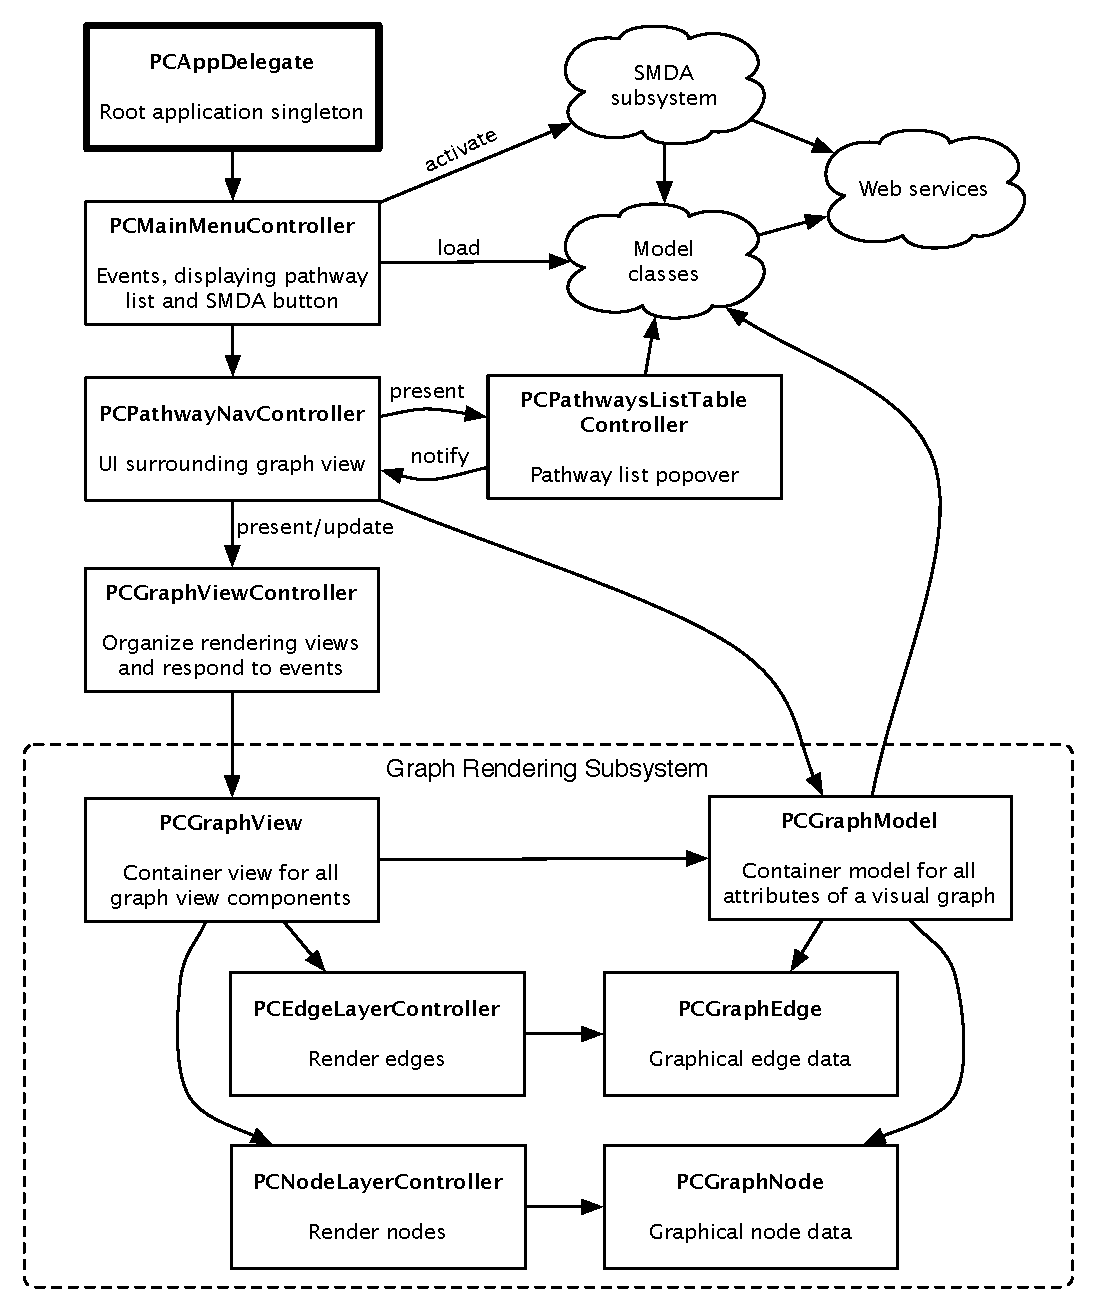
\includegraphics[width=5in]{figures/components.pdf}}
    \caption{\label{fig:components} Components of the architecture}
\end{figure}

The application is divided into several classes. The relationships between them are represented in three figures. Figure \ref{fig:components} shows references between instances. Figure \ref{fig:controlflow} shows the flow of control in response to events from the event loop. Figure \ref{fig:dataflow} shows the flow of data between the methods involved in loading and displaying a graph.

\texttt{PCAppDelegate} handles application-level delegate methods and notifications from the system.  \texttt{PCGraphViewController}, associated with \texttt{GraphView.xib}, ties together all user interface elements. There are currently only two interactive elements, the graph view and the ``Pathways'' button on the toolbar.

The Pathways button causes a popover list of available pathways to be displayed. This popover is populated by \texttt{PCPathwayListTableController}. When one of these pathway names is clicked, an event is sent back to \texttt{PCGraphViewController}, which requests graph data from the PathCase server. This data is parsed by \texttt{PCGraphModel}, \texttt{PCGraphNode}, and \texttt{PCGraphEdge} into renderable objects.

The \texttt{PCGraphModel} is attached to a \texttt{PCGraphView} which puts the graphics data into a series of nested layers and provides it to a \texttt{UIScrollView}, a Cocoa object which provides panning and zooming.

\begin{figure}[htb]
    \center{
        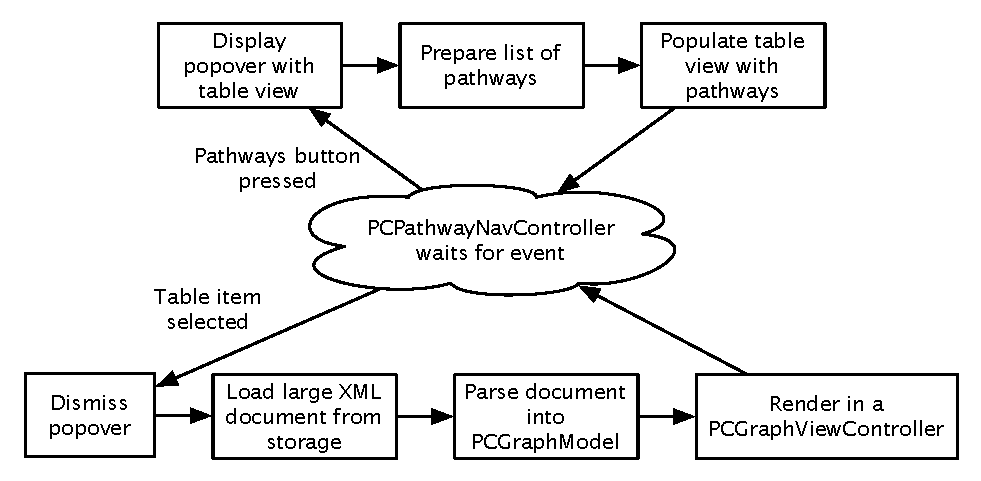
\includegraphics[width=4.5in]{figures/controlflow.pdf}}
    \caption{\label{fig:controlflow} Control flow for displaying graphs}
\end{figure}

\begin{figure}[htb]
    \center{
        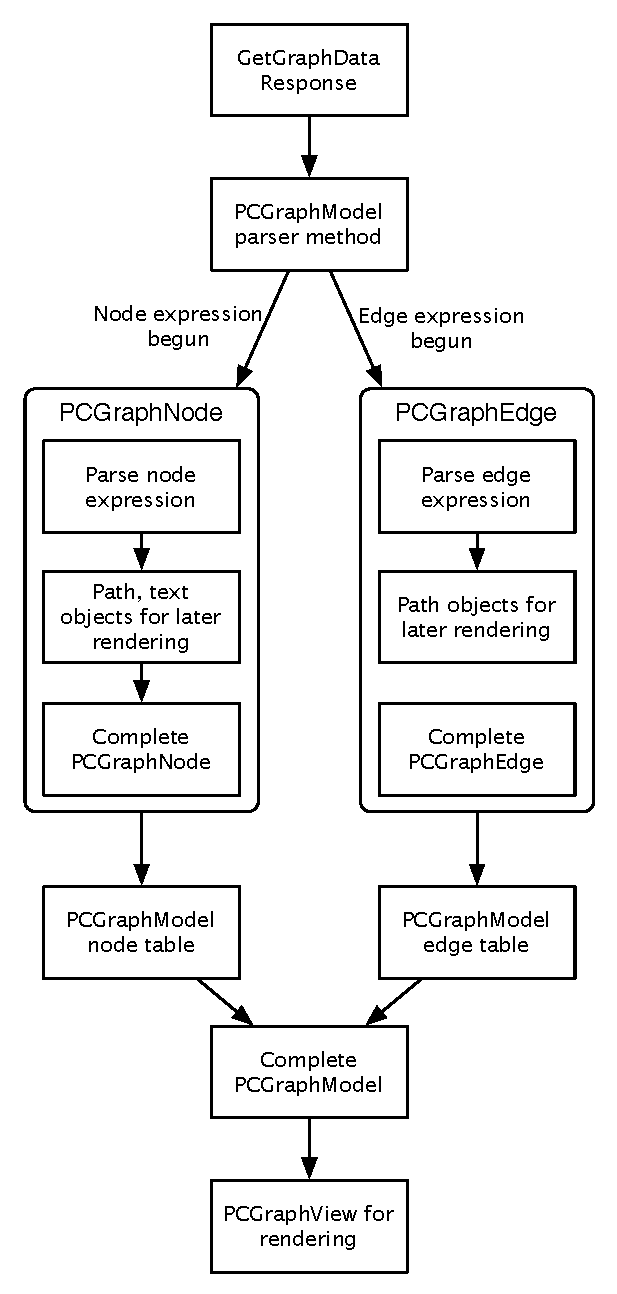
\includegraphics[width=3in]{figures/dataflow.pdf}}
    \caption{\label{fig:dataflow} Data flow for graph data}
\end{figure}
